\chapter{Introduction}
\label{sec:introduction}

Rotary wing micro aerial vehicles (MAVs) have been well studied in academia
and found a lot of applications in the world such as search operations
\citep{silvagni_multipurpose_2017}, photography \citep{noauthor_dji_nodate} or
even toys \citep{noauthor_aura_nodate}. They encountered such a broad success because
of their agility and mechanical simplicity. Nevertheless, traditional multi-rotor
vehicles are under-actuated, which means that they cannot control their torque
and force independently \citep{brescianini_design_2016}. They are thus unable to
change their position without changing their orientation. \\
Recently the focus has been on designing MAVs able to perform more complex
tasks such as camera motion for the film industry \citep{kamel_voliro:_2018} or
bridge inspection where huge resources (i.e. cranes and large man-power)
are needed. The ultimate goal would be for a drone to be able to interact with
its surrounding and apply forces to it, in order to perform maintenance where
humans can not access, or to do construction work in harsh environments. \\
To perform these tasks, an MAV has to be able to hover in any orientation, and for a
proper disturbance rejection while manipulating, the drone must have the potential
to accelerate instantaneously in any direction. Hence, the MAV has to be able to
decouple its orientation and position control. A drone that has a decoupled
force and torque control is referred to as an omni-directional MAV. \\
The problem of overcoming the under-actuation and achieving omni-directionality
is not straightforward. To address this problem, several MAV designs have been
presented over the past years. For instance, in \citep{kamel_voliro:_2018}, Voliro
(name of the vehicle) is based on a traditional hexa-copter (see \Cref{fig:voliro}).
The omni-directionality issue is addressed by adding motors to rotate the
thrusters around their arm axis, thus allowing a control not only of the thrust
produced by each propeller, but also of the orientation of this thrust. This
tilting rotor system allows for decoupling the control of position and orientation.
By using a control scheme based on an allocation technique, the system provides
very good maneuverability.

\begin{figure}[h]
\centering
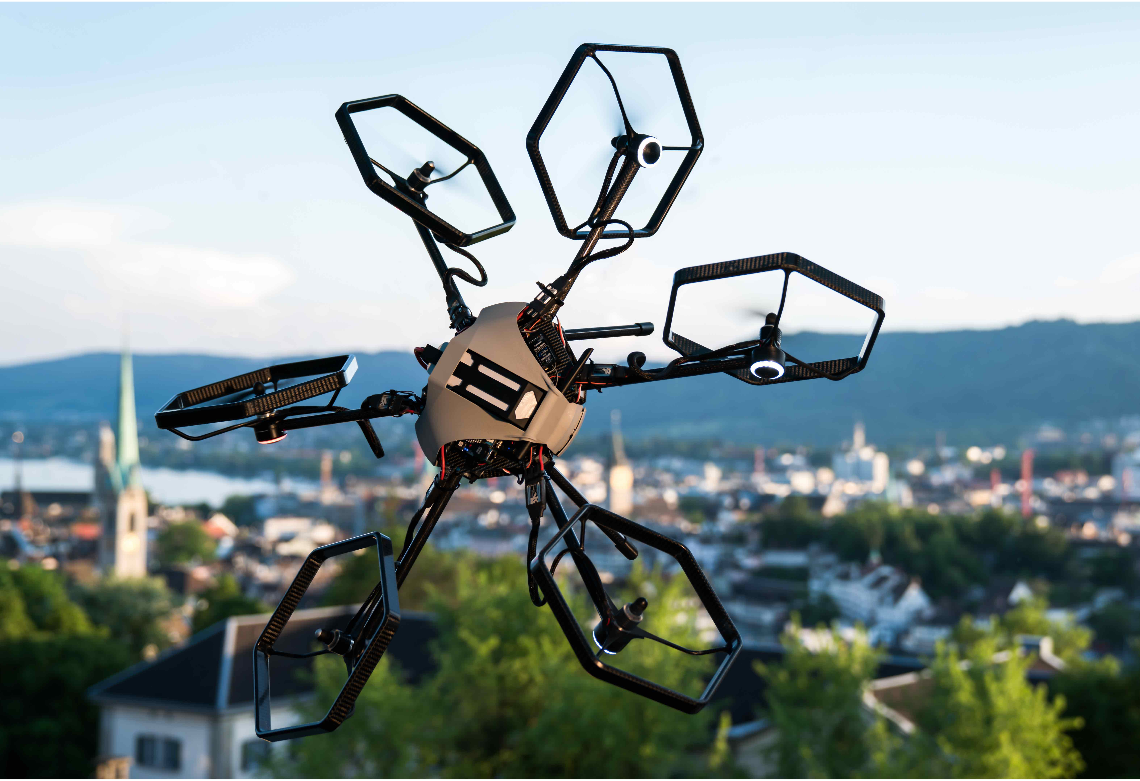
\includegraphics[width=0.4\textwidth]{images/voliro.png}
\caption{Voliro \citep{kamel_voliro:_2018}.}
\label{fig:voliro}
\end{figure}

In \citep{brescianini_design_2016}, the Omnicopter (name of the vehicle) is described.
It is a drone with eight fixed rotors and the drone shape is the result of a mathematical
optimization which maximizes the vehicle’s agility with the constraint that its
dynamical properties would be as independent as possible on the vehicle's orientation
(see \Cref{fig:omnicopter}).

\begin{figure}[h]
\centering
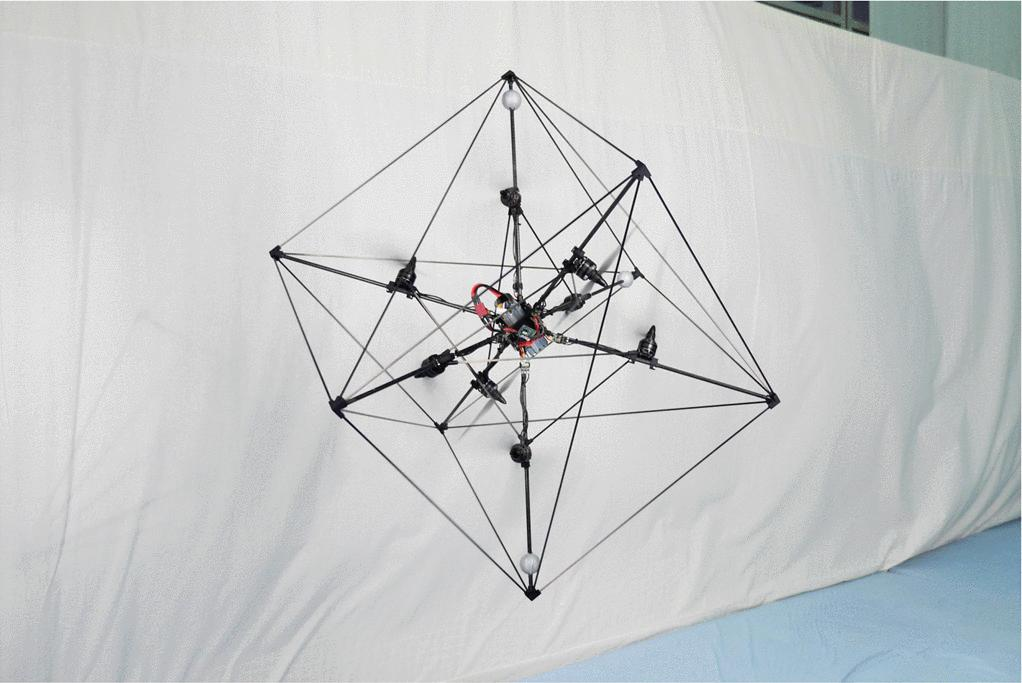
\includegraphics[width=0.4\textwidth]{images/idsc.jpg}
\caption{Ominicopter \citep{brescianini_design_2016}.}
\label{fig:omnicopter}
\end{figure}

In \citep{nikou_mechanical_2015}, the MAV is a fixed propeller multi-rotor.
The design is also the result of an optimization, which tends to minimize the
body volume, to maximize the controllability of the system, avoid eventual
aerodynamic interactions and to maximizes the efficiency in performing
manipulation tasks. \\
The idea presented in \citep{rajappa_modeling_2015} is a mix between
Voliro and the Omnicopter because the design is a modified hexarotor,
which achieves full control over the vehicle’s position and orientation using
manually tiltable propellers (see \Cref{fig:hexacopter}). The paper also provides
a methodology to optimize the fixed tilting angles depending on the desired trajectory.

\begin{figure}[h]
  \centering
  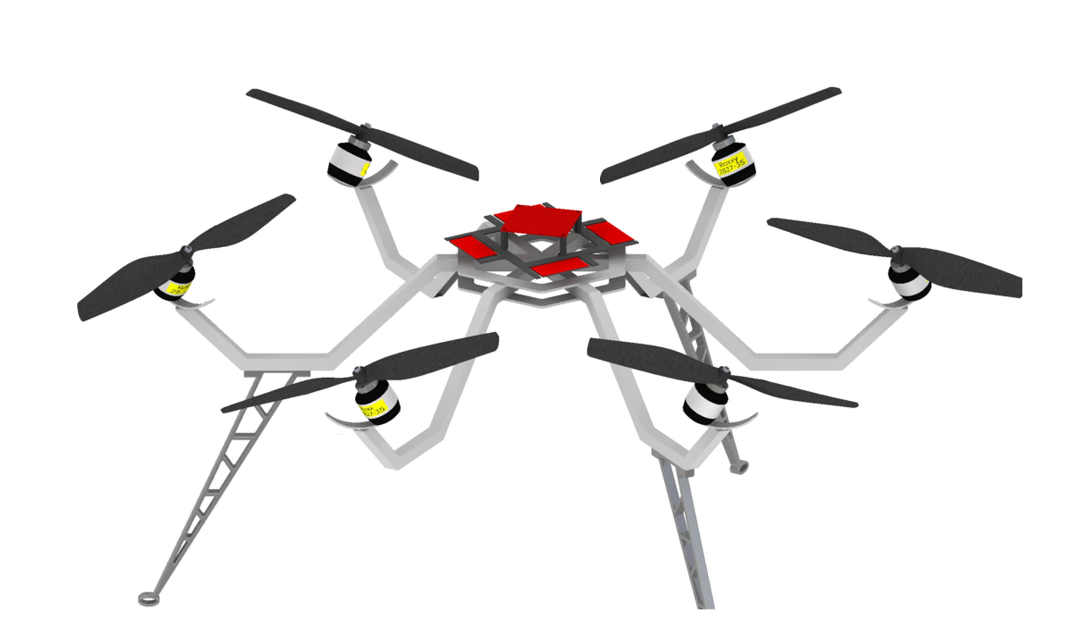
\includegraphics[width=0.4\textwidth]{images/hexacopter.png}
  \caption{Hexacopter with manually tiltable rotors \citep{rajappa_modeling_2015}.}
  \label{fig:hexacopter}
\end{figure}

Yet, nothing in the literature is found about the morphology optimization
of MAVs with tilting rotors. Hence the need for the present research project.
The aim of this thesis is thus to design a morphology optimization problem for
a tilt-rotor MAV that accounts for the different factors that influence the
morphology such as:

\begin{itemize}
\item Omni-directionality
\item Flight efficiency
\item Controlability
\end{itemize}

To reach this goal the chosen approach is to build an optimization tool that solves
the optimization problem and returns different MAV designs. The most interesting
designs are then tested in simulation.
In this report the methods used to build the optimization tool and to simulate
the results are discussed. Afterwards, the results returned by the tool are shown
and compared based on different criteria. Finally, the results gathered during
the simulation phase are also covered.
